\chapter{Experiments}\label{C:experiments}

\section{Introduction}

All the algorithms above excluding DQN can work on continuous action spaces. This makes them suited for continuous control tasks that are common within the robotic control domain. I will conduct experiments using the Gymnasium \cite{towers2024gymnasium} library which provides a framework to use among other things some Mujoco \cite{todorov2012mujoco} environments. Specifically I will use \texttt{Humanoid-v5, HumanoidStandup-v5, Walker2d-v5, Ant-v5, HalfCheetah-v5} and \texttt{Hopper-v5} which cover a range of locomotion tasks. \dots

\section{Baseline Experiments}

I will look at two things for ll of my baseline algorithms. The first is the sample efficiency and the second is the computational efficiency.

\subsection{Sample Efficiency}
To measure the sample efficient I will look at the average reward over 10 episodes every 1000 steps. This will give a learning curve to demonstrate how effective its actions are given how many interactions it has had with the environments.

\begin{figure}[H]
    \centering
    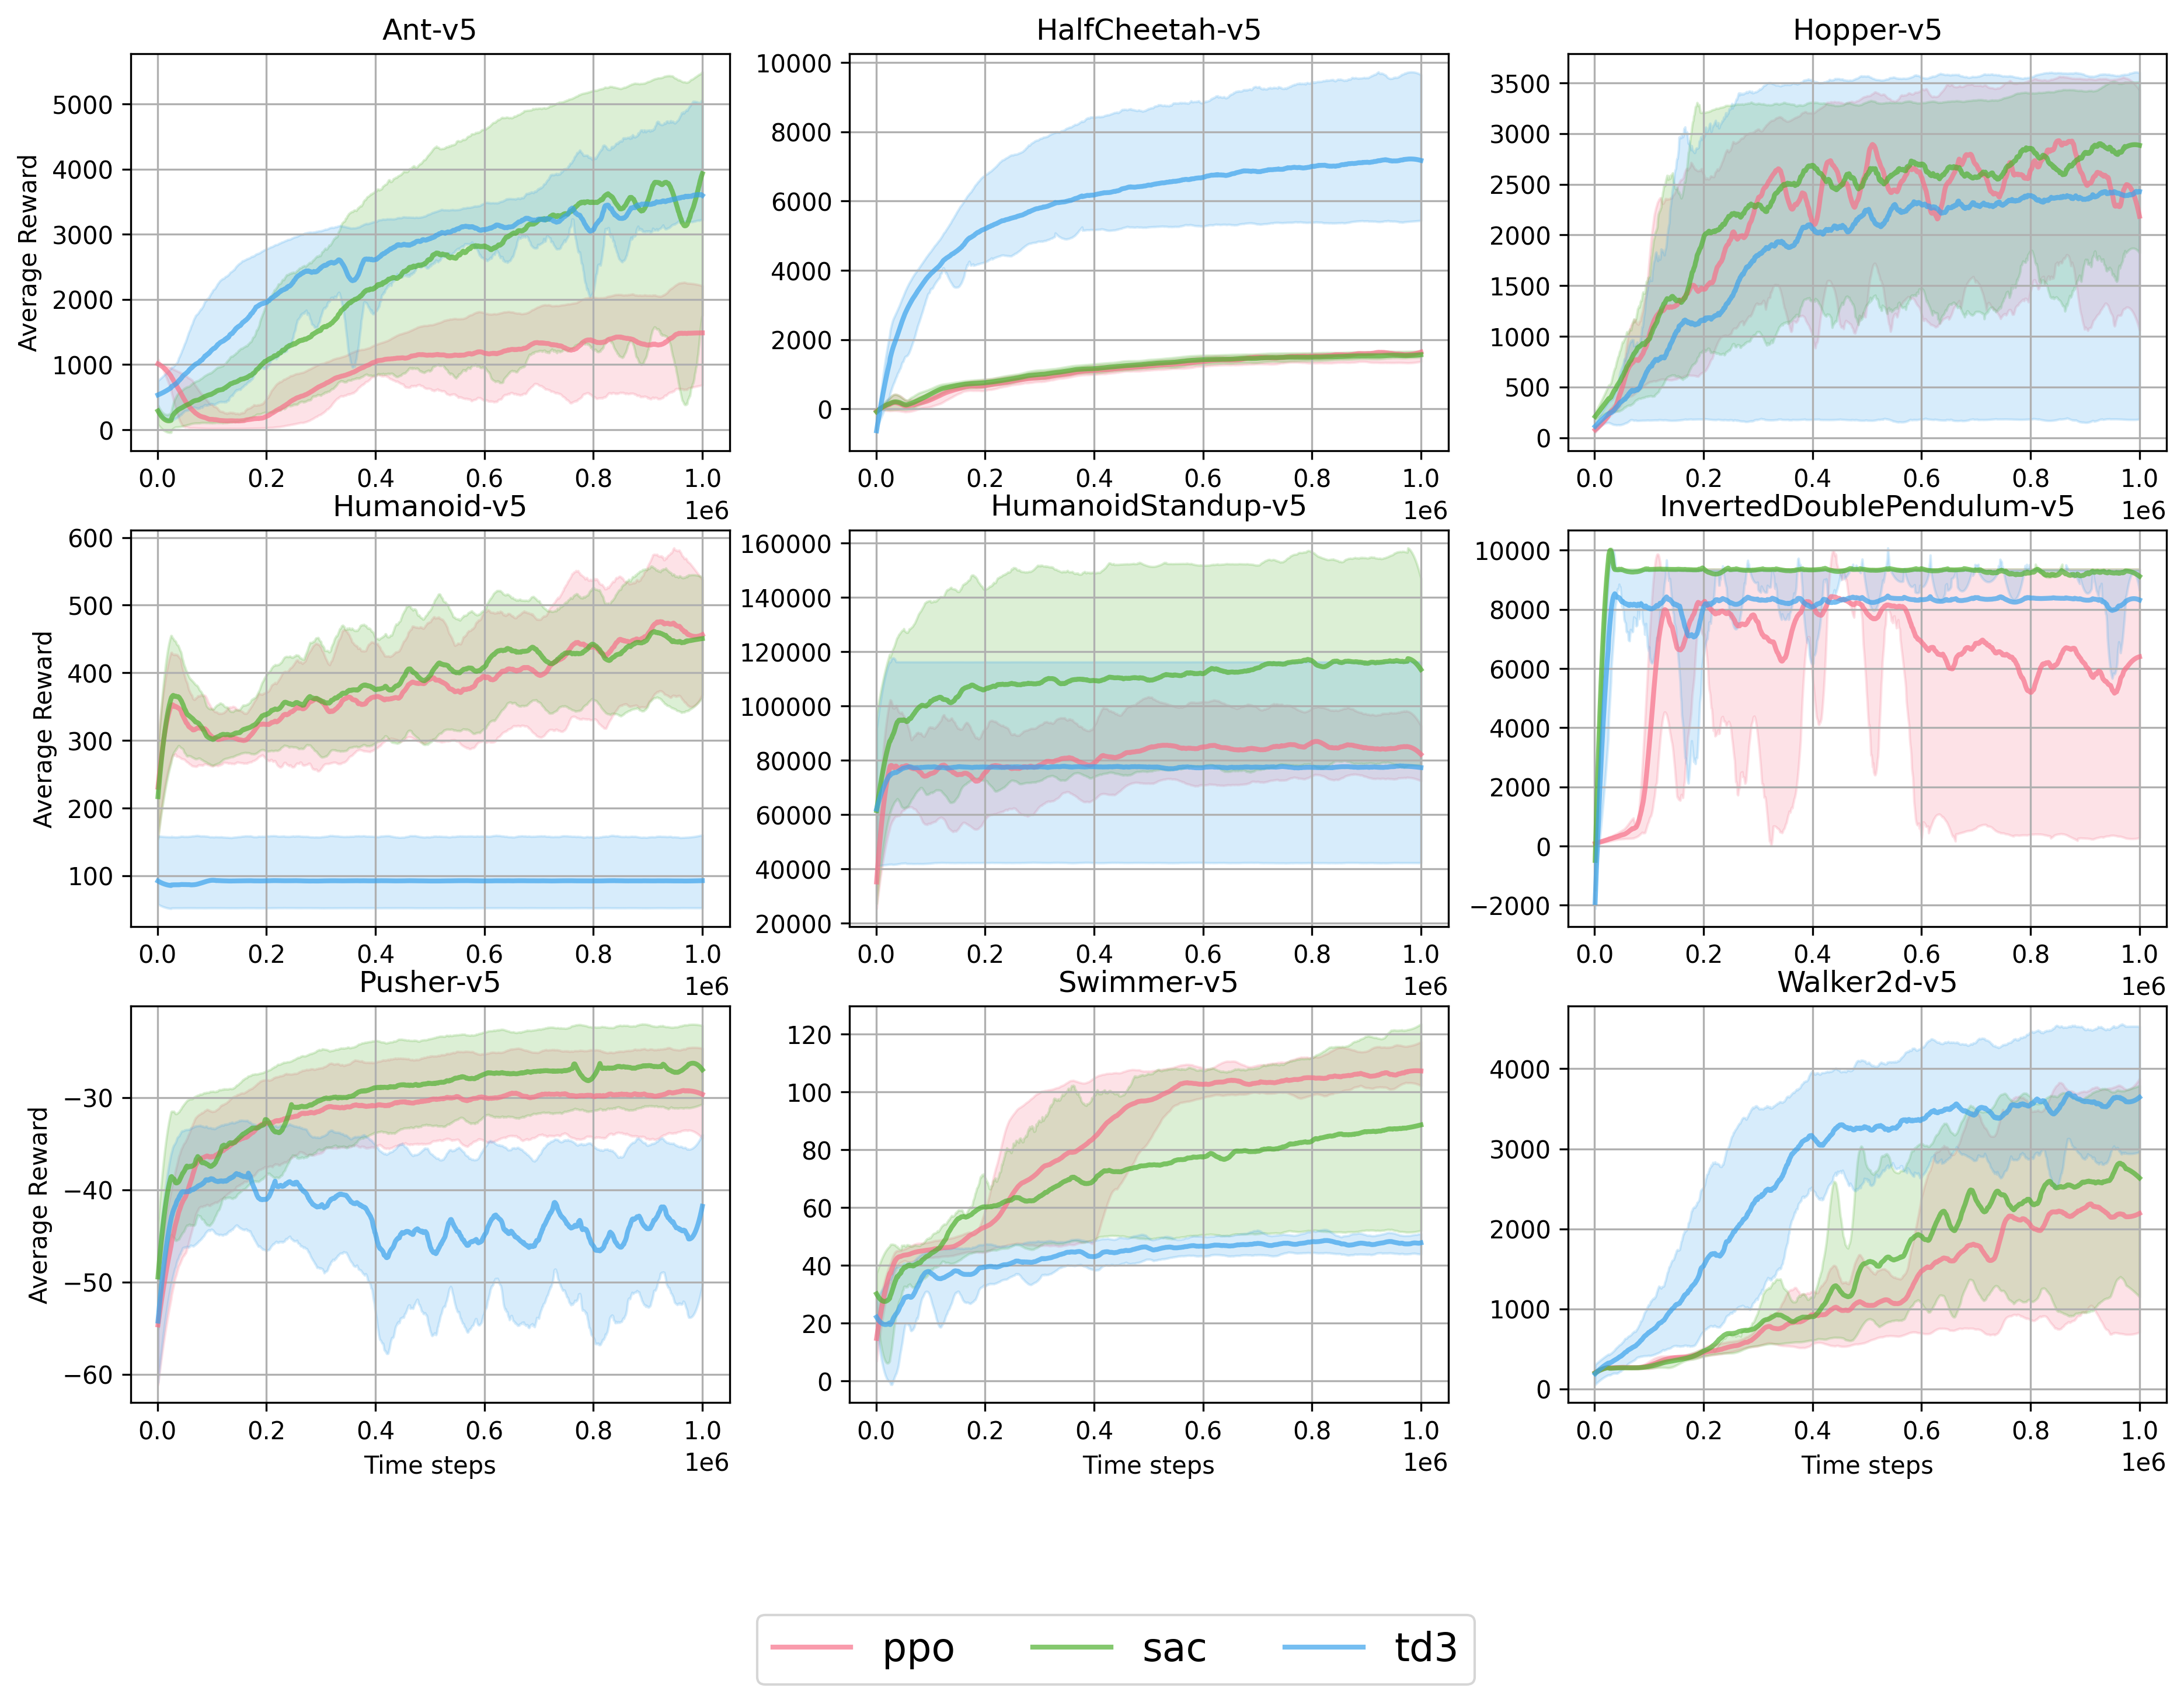
\includegraphics[width=1\textwidth]{figures/baseline_results.png}
    \caption{Sample Efficiency of PPO, SAC, TD3, TQC, REDQ, CrossQ and DroQ.}
    \label{fig:sample_efficiency}
\end{figure}

Information on the implementations of the algorithms and the hyperparameters can be found in appendix \ref{C:appendixA}.

\textit{Simple analysis of the results here}

\dots

\subsection{Computational Efficiency}

The measure of computational efficiency is about measuring the amount of computation it takes to get a an agent to learn a certain task. As there is a variety of different algorithms the mos general method is to measure the wall clock time it takes the algorithm to complete a certain number of environment steps.

\textit{figure here}

All of experiments were run on \dots

\dots
